\documentclass[8pt]{article}
\usepackage[UTF8]{ctex}
\usepackage[a4paper]{geometry}

\usepackage{amsthm,amsmath,amssymb}
\usepackage{graphicx}
\usepackage{subfigure}
\usepackage{amsmath}
\usepackage{tabularx}
\usepackage{color}
\usepackage{hyperref}
\usepackage{ulem}
\usepackage{multirow}
\usepackage[cache=false]{minted}
\hypersetup{
	colorlinks=true,
	linkcolor=blue
}

\usepackage{appendix}
\geometry{a4paper,centering,scale=0.8}
\geometry{left=2.0cm, right=2.0cm, top=2.5cm, bottom=2.5cm}
\usepackage[format=hang,font=small,textfont=it]{caption}
\usepackage[nottoc]{tocbibind}

\usepackage{algorithm}
\usepackage{algorithmicx}
\usepackage{algpseudocode}
\usepackage{amssymb}
\usepackage{extarrows}
\usepackage{qcircuit}
\usepackage{fancyhdr}
\usepackage{fancyvrb}

\fvset{showspaces=true}
\SaveVerb{verbspace}! !
\newcommand{\aspace}{\UseVerb{verbspace}}%
\usepackage{cleveref}

\usepackage{pgf}
\usepackage{totpages}
\usepackage{tikz}  
\usetikzlibrary{arrows,automata}

\usetikzlibrary{arrows.meta}%画箭头用的包

\makeatletter
\def\@maketitle{%
	\newpage
	\begin{center}%
		\let \footnote \thanks
		{\LARGE \@title \par}%
		\vskip 1.5em%
		{\large
			\lineskip .5em%
			\begin{tabular}[t]{c}%
				\@author
			\end{tabular}\par}%
		\vskip 1em%
		{\large \@date}%
	\end{center}%
	\par
	\vskip 1.5em}
\makeatother

\newtheoremstyle{compact}%
{3pt}{3pt}%
{}{}%
{\bfseries}{\textcolor{red}{.}}%  % Note that final punctuation is omitted.
{.5em}{\mbox{\textcolor{red}{\thmname{#1}\thmnumber{ #2}}\thmnote{ (\textcolor{blue}{#3})}}}
\theoremstyle{compact}
\newtheorem{innercustomgeneric}{\customgenericname}
\providecommand{\customgenericname}{}
\newcommand{\newcustomtheorem}[2]{%
	\newenvironment{#1}[1]
	{%
		\renewcommand\customgenericname{#2}%
		\renewcommand\theinnercustomgeneric{##1}%
		\innercustomgeneric
	}
	{\endinnercustomgeneric}
}

\DeclareMathOperator{\card}{card}

\newtheorem{theorem}{定理}
\newtheorem{lemma}{引理}
\newtheorem{definition}{定义}
\newtheorem{proposition}{命题}
\newtheorem{corollary}{推论}
\newtheorem{example}{例}
\newtheorem{claim}{声明}
\newtheorem{remark}{注}
\newtheorem{thesis}{论点}
\newtheorem{Proof}{证明}

\def\obj#1{\textbf{\uline{#1}}}
\def\num#1{\textnormal{\textbf{\mbox{\textcolor{blue}{(#1)}}}}}
\def\le{\leqslant}
\def\ge{\geqslant}
\def\im{\text{im }}
\def\Pr#1{\text{Pr}\left[{#1}\right]}
\def\E#1{\mathbb{E}\left[{#1}\right]}
\def\Var#1{\text{Var}\left[{#1}\right]}
\def\rep#1{\llcorner{#1}\lrcorner}

\def\DTIME{\textbf{DTIME}}
\def\NTIME{\textbf{NTIME}}
\def\P{\textbf{P}}
\def\NP{\textbf{NP}}
\def\EXP{\textbf{EXP}}
\def\SPACE{\textbf{SPACE}}
\def\NSPACE{\textbf{NSPACE}}
\def\PSPACE{\textbf{PSPACE}}
\def\NPSPACE{\textbf{NPSPACE}}
\def\L{\textbf{L}}
\def\NL{\textbf{NL}}


\title{\heiti\zihao{1} 计算理论导论\ 课程讲义}
\author{\kaishu\zihao{-3} 酥雨\\zusuyu@stu.pku.edu.cn}

\CTEXoptions[today=old]
\date{\today}

\begin{document}
\fancypagestyle{plain}{
	\fancyhf{}
	\lhead{Introduction to the Theory of Computation}
	\chead{2022 Spring}
	\rhead{计算理论导论\ 课程笔记}
	\cfoot{第 \thepage 页, 共 \pageref{TotPages} 页}
}
\pagestyle{plain}

\crefname{theorem}{定理}{定理}
\crefname{lemma}{引理}{引理}
\crefname{proposition}{命题}{命题}
\crefname{figure}{图}{图}
\crefname{table}{表}{表}	
\maketitle

\section*{Outline}
	\begin{enumerate}	
		\item DFA/NFA, Regular Language, Pumping Lemma
		\item Context-free Language, Pumping Lemma
		\item Turing Machine
		\item Undecidable Language
		\item Time Complexity \P\ and \NP
		\item Space Complexity \PSPACE, \L\ and \NL
		\item Polynomial Hierarchy
		\item Circuit Complexity
		\item Random Computation
		\item Interactive Proof
		\item (optional) Crypt, Quant, Learning
	\end{enumerate}



\newpage
\section{正则语言}
\begin{definition}[Deterministic Finite Automaton, DFA]
	(确定性)有限自动机是一个五元组$(Q, \Sigma, \delta, q_0, F)$, 其中
	\begin{itemize}
		\item $Q$是称为\obj{状态}的有限集. 
		\item $\Sigma$是称为\obj{字符集}的有限集. 
		\item $\delta: Q \times \Sigma \to Q$被称为\obj{转移函数}. 
		\item $q_0 \in Q$称为\obj{起始态}. 
		\item $F \subseteq Q$称为\obj{接受态(终止态)集合}. 
	\end{itemize}

	称字符串$w = w_1w_2\cdots w_m(w_i \in \Sigma)$可以被DFA $M = (Q, \Sigma, \delta, q_0, F)$接受, 如果存在状态序列$r_0, r_1, \cdots, r_m \in Q$满足\num{i}$r_0 = q_0$, \num{ii}$r_{i+1} = \delta(r_i, w_{i+1}) \ (\forall i = 0, 1, \cdots, m-1)$, \num{iii}$r_m \in F$. 

	所有可被$M$识别的字符串$w$构成集合$A$, 则称$A$是 DFA $M$的语言(或者说 DFA $M$识别/接受$A$), 记为$L(M) = A$.
\end{definition}
\begin{definition}[正则语言]
	正则语言就是能够被有限自动机识别的语言. 
\end{definition}
\begin{definition}[正则操作]
	定义如下三种正则操作
	\begin{itemize}
		\item \obj{Union}: $A \cup B = \{x | x \in A \textrm{ or } x \in B\}$.
		\item \obj{Concatenation}: $A \circ B = \{xy | x \in A \textrm{ and } y \in B\}$.
		\item \obj{Star}: $A^* = \{x_1x_2\cdots x_k | k \ge 0 \textrm{ and each } x_i \in A\}$.
	\end{itemize}
\end{definition}
\begin{remark}
	补集$\overline{A} = \Sigma^* - A$操作在正则语言下是封闭的: 只需要把终止态集合$F$改成$Q - F$即可.
\end{remark}
\begin{theorem}
	正则操作 union 在正则语言下是封闭的: 把两个自动机放在一起跑就行了. 
\end{theorem}
由于只利用已有的有限自动机模型证明 concatenation 和 star 的封闭性是困难的, 我们引入“非确定性”. 
\begin{definition}[Nondeterministic Finite Automaton, NFA]
	非确定性有限自动机是一个五元组$(Q, \Sigma, \delta, q_0, F)$, 其中$\delta$不再是$Q \times \Sigma \to Q$的函数, 而是$Q \times \Sigma_{\varepsilon} \to \mathcal P(Q)$的, 其中$\mathcal P$表示幂集, $\Sigma_{\varepsilon}$表示$\Sigma \cup \{\varepsilon\}$. 

	相应的, 称字符串$w = w_1w_2\cdots w_m(w_i \in \Sigma)$可以被NFA $N = (Q, \Sigma, \delta, q_0, F)$接受, 如果$w$可以写成$w = y_1y_2\cdots y_{m'}(y_i \in \Sigma_{\varepsilon})$, 且存在状态序列$r_0, r_1, \cdots, r_{m'} \in Q$满足\num{i}$r_0 = q_0$, \num{ii}$r_{i+1} \in \delta(r_i, y_{i+1})$\ $(\forall i = 0, 1, \cdots, {m'}-1)$, \num{iii}$r_{m'} \in F$. 
\end{definition}
\begin{remark}
	DFA的每个状态对每种字符都有恰好一条转移出边, 而相对的, NFA可能有零条、一条或者多条, 有几条出边就表示会创建出多少个独立的“后继进程”. 此外还存在$\varepsilon$的出边, 表示可以不输入任何字符创建进程. 
\end{remark}
\begin{theorem}[NFA与DFA的等价性]
	任何NFA都存在等效的DFA. 
\end{theorem}
\begin{proof}
	对$k$个状态的NFA, 构造一个$2^k$个状态的DFA, 每个状态表示“可能处在的NFA状态”的子集. 

	形式化的, 对于 NFA $M = (Q, \Sigma, \delta, q_0, F)$, 构造 DFA $M' = (Q', \Sigma, \delta', q_0', F')$, 其中
	\begin{itemize}
		\item $Q' = \mathcal P(Q)$.
		\item $\forall R \in Q', a \in \Sigma, \delta'(R, a) = \bigcup_{r \in R}\delta(r, a)$.
		\item $q_0' = \{q_0\}$.
		\item $F' = \{R \in Q' | R \cap F \neq \varnothing\}$.
	\end{itemize}
\end{proof}
\begin{corollary}
	一个语言是正则的当且仅当可以被一台非确定性有限自动机识别. 
\end{corollary}
\begin{theorem}
	union, concatenation 和 star 在正则语言下都是封闭的. 
\end{theorem}
\begin{proof}
	不多说了看图. 

	\begin{figure}[htbp]
		\centering
		\subfigure[proof for union]{
			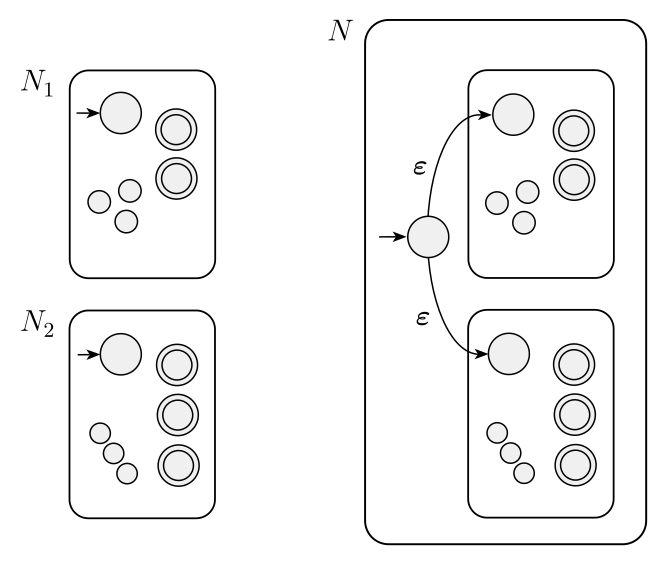
\includegraphics[scale=0.25]{pic/union.png}
		}
		\quad
		\subfigure[proof for concatenation]{
			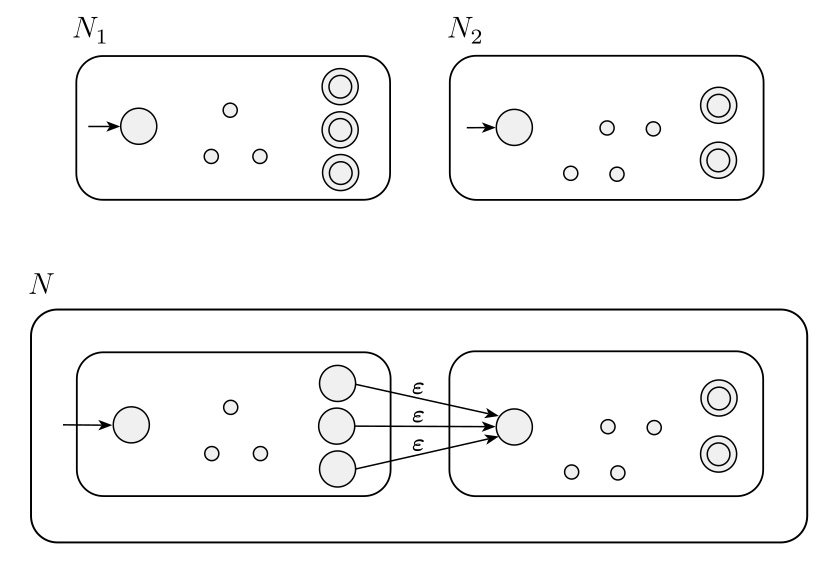
\includegraphics[scale=0.25]{pic/concat.png}
		}
		\quad
			\subfigure[proof for star]{
			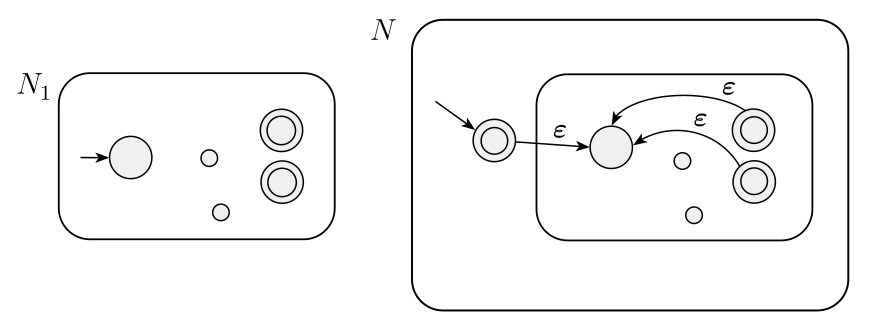
\includegraphics[scale=0.25]{pic/star.png}
		}
	\end{figure}
\end{proof}
\begin{definition}[正则表达式]
	称$R$是正则表达式, 如果$R$为
	\begin{itemize}
		\item $\{a\}$, 其中$a$是字符集$\Sigma$中的某个元素
		\item $\{\varepsilon\}$, 其中$\varepsilon$表示空串
		\item $\varnothing$
		\item $(R_1 \cup R_2)$, 其中$R_1, R_2$是某两个正则表达式
		\item $(R_1 \circ R_2)$, 其中$R_1, R_2$是某两个正则表达式
		\item $(R_1^*)$, 其中$R_1$是某个正则表达式
	\end{itemize}
\end{definition}
\begin{example}
	对于任意正则表达式$R$, $R \cup \varnothing = R \circ \varepsilon = R$, $R \circ \varnothing = \varnothing$, $\varnothing^* = \{\varepsilon\}$. 
\end{example}
\begin{theorem}[正则表达式与有限自动机的等价性]
	一个语言是正则的当且仅当它可以被一个正则表达式描述. 
\end{theorem}
\begin{proof}
	“$\Leftarrow$”的证明是简单的, 只需要根据正则表达式$R$构造NFA, 利用“union, concatenation, star的封闭性”的构造性证明即可. 

	“$\Rightarrow$”的证明中, 我们引入GNFA的定义(每条转移边上的label是一个正则表达式), 然后分别展示如何把DFA转化成GNFA以及如何根据GNFA构造正则表达式. 

	DFA转GNFA是简单的——只需要额外加入两个状态表示$q_{\text{start}}$和$q_{\text{accept}}$即可. 

	观察到一个GNFA有$k \ge 2$个状态. 如果$k=2$, 那么$q_{\text{start}}$到$q_{\text{accept}}$的转移边上的正则表达式就是该有限自动机对应的正则表达式. 如果$k > 2$, 那么考虑选出一个状态$q_{\text{rip}}$删除, 此时对于$q_i, q_j \in Q \setminus \{q_{\text{rip}}\}$, 如果$\delta(q_i,  q_{\text{rip}}) = R_1, \delta(q_{\text{rip}}, q_{\text{rip}}) = R_2, \delta(q_{\text{rip}}, q_j) = R_3, \delta(q_i, q_j) = R_4$, 则修改$\delta'(q_i, q_j) = (R_1)(R_2)^*(R_3) \cup (R_4)$. 归纳即可. 
\end{proof}
\begin{definition}[Generalized Nondeterministic Finite Automaton, GNFA]
	广义非确定性有限自动机是一个五元组$(Q, \Sigma, \delta, q_{\text{start}}, q_{\text{accept}})$, 其中$\delta$是$(Q \setminus \{q_{\text{accept}}\}) \times (Q \setminus \{q_{\text{start}}\}) \to \mathcal R$的转移函数, $\mathcal R$表示字符集$\Sigma$上的所有正则表达式. 注意不失一般性地要求了只有唯一的接受态, 以及$q_{\text{start}} \neq q_{\text{accept}}$. 
\end{definition}
\begin{theorem}[Pumping Lemma for Regular Language]
	如果$A$是正则语言, 那么存在一个数$p$ (称为\obj{pumping length}), 使得对于任意$A$中长度至少为$p$的字符串$s$, $s$都可分成三部分$s = xyz$满足
	\begin{itemize}
		\item for each $i \ge 0$, $xy^iz \in A$,
		\item $|y| > 0$,
		\item $|xy| \le p$.
	\end{itemize}
\end{theorem}
\begin{proof}
	取 pumping length $p$ 为识别此正则语言的 DFA $M$的状态集大小$|Q|$. 对于任意长度至少为$p$的$s \in A$, 其经过的状态序列至少长为$p+1$. 根据\obj{鸽巢原理}, 存在一个状态$q$经过了至少两次, 于是把从$q_{\text{start}}$走到$q$的部分视作$x$, $q$回到自身的环视作$y$, 从$q$走到$q_{\text{accept}}$的部分视作$z$, 便构造出了划分. 
\end{proof}
\begin{remark}
	利用 pumping lemma 可以证明某个语言$B$不是正则语言, 通用的方式是:先假设$B$是正则的, 导出 pumping length $p$的存在性, 然后根据这个$p$构造$s \in B$, 并验证其\obj{不能}被划分为$s = xyz$. 第三个条件$|xy| \le p$有时也是有用的. 
\end{remark}
\begin{example}
	$B = \{0^n1^n | n \ge 0\}$ 不是正则语言.
\end{example}
\begin{proof}
	假设 $B$ 是正则语言, 那么就存在 pumping length $p$. 考虑串 $0^p1^p$, 无论 $y$ 取其何种子串, $xyyz$ 都不可能 $\in B$. 因此 $B$ 不是正则语言.
\end{proof}
\begin{example}
	$C = \{w | w \text{ has an equal number of 0s and 1s}\}$ 不是正则语言.
\end{example}
\begin{proof}
	假设 $C$ 是正则语言, 那么就存在 pumping length $p$. 考虑串 $0^p1^p$, 注意到我们要求了 $|xy| \le p$, 所以 $y$ 只能包含 $0$, 此时 $xyyz \notin B$. 因此 $C$ 不是正则语言.
	
	\textit{另一种证法是: 考虑 $C \cap 0^*1^* = B$, 正则语言在 intersection 下是封闭的, 所以$C$正则会导出$B$正则.}
\end{proof}
\begin{example}
	$F = \{ww | w \in \{0, 1\}^*\}$ 不是正则语言.
\end{example}
\begin{proof}
	考虑串 $0^p10^p1$, 注意到 $y$ 只能包含 $0$, 从而$xyyz \notin F$, 因此$F$不是正则语言.
\end{proof}

\begin{example}
	$D = \{1^{n^2} | n \ge 0\}$ 不是正则语言.
\end{example}
\begin{proof}
	考虑串 $1^{p^2}$. 由于 $|y| \le p$, 所以 $|xyyz| = p(p+1) < (p+1)^2$ 不可能是完全平方数, $xyyz \notin D$, 说明$D$不是正则语言.
\end{proof}
\begin{example}
	$E = \{0^i1^j | i > j\}$不是正则语言. 
\end{example}
\begin{proof}
	考虑串$0^{p+1}1^p$, $y$只能包含 $0$, 且$|y| > 0$, 因此$xz$中$0$的个数不超过 $1$的个数, $xz \notin E$, 说明 $E$ 不是正则语言.
\end{proof}
\newpage
\section{上下文无关文法}
\begin{definition}[Context-Free Grammar/Language, CFG/CFL]
	一个上下文无关文法是一个四元组$(V, \Sigma, R, S)$, 其中
	\begin{itemize}
		\item $V$是称为\obj{变量}的有限集, 
		\item $\Sigma$是称为\obj{终止符}的有限集, 与$V$不交, 
		\item $R$是称为\obj{规则}的有限集, 是从$V$到$(V \cup \Sigma)^*$的映射, 
		\item $S \in V$称为\obj{起始变量}. 
	\end{itemize}

	上下文无关语言就是上下文无关文法导出/生成的语言, 即$\{w \in \Sigma^* | S \overset{*}{\Rightarrow} w\}$. 
\end{definition}
\begin{definition}[parse tree]
	形如这样子的东西.
	\begin{center}
		\includegraphics*[scale=0.4]{pic/parse_tree.png}	
	\end{center}
\end{definition}
\begin{proposition}
	CFG 的描述能力严格强于有限自动机(或者正则表达式). 
\end{proposition}
\begin{proof}
	对于任意的DFA, 都可以构造与其等价的CFG:对每个状态$q_i$构造一个变量$R_i$, 起始变量$R_0$对应起始态$q_0$, 如果$\delta(q_i, a) = q_j$, 就添加规则$R_i \to aR_j$, 而如果$q_i$是接受态, 就添加规则$R_i \to \varepsilon$. 

	而显然存在可被 CFG 描述的非正则语言, 比如$\{0^n1^n | n \in \mathbb N\}$. 
\end{proof}
\begin{definition}[歧义性]
	称一个串 $w$ 由 CFG $G$ 歧义生成, 如果存在 $G$ 下 $w$ 的两种 lestmost derivation (每次只替换最左边的变量)方式, 或者说存在两棵不同的 parse tree 可以生成 $w$. 称一个 CFG $G$ 是歧义的, 如果它可以歧义生成某些串.
\end{definition}
\begin{definition}[固有歧义]
	称一个 CFL $L$ 是固有歧义的, 如果 $L$ 只能由歧义的 CFG $G$ 生成.
\end{definition}
\begin{example}
	$\{a^ib^jc^k | i = j \textrm{ or } j = k\}$ 是固有歧义的.
\end{example}
\begin{definition}[Pushdown Automaton, PDA]
	下推自动机是一个六元组$(Q, \Sigma, \Gamma, \delta, q_0, F)$, 其中
	\begin{itemize}
		\item $Q$是状态集, 
		\item $\Sigma$是输入字符集, 
		\item $\Gamma$是栈字符集, 
		\item $\delta: Q \times \Sigma_{\varepsilon} \times \Gamma_{\varepsilon} \to \mathcal P(Q \times \Gamma_{\varepsilon})$是转移函数, 
		\item $q_0 \in Q$是起始态, 
		\item $F \subseteq Q$是接受态集合. 
	\end{itemize}

	其中$\Sigma_{\varepsilon}, \Gamma_{\varepsilon}$分别表示$\Sigma \cup \{\varepsilon\}, \Gamma \cup \{\varepsilon\}$. $(q', b) \in \delta(q, c, a)$ 表示在状态 $q$ 上被输入 $c$ 字符时, 会先从栈顶 pop 出字符 $a$, 再向栈顶 push 进字符 $b$, 最后转移到状态 $q'$. 幂集$\mathcal P$暗含了下推自动机是 nondeterministic 的. 

	称字符串$w = w_1w_2\cdots w_m(w_i \in \Sigma_{\varepsilon})$可以被 PDA $M = (Q, \Sigma, \Gamma, \delta, q_0, F)$接受, 如果存在状态序列$r_0, r_1, \cdots, r_m \in Q$和字符串(栈)序列$s_0, s_1, \cdots, s_m \in \Gamma^*$, 满足
	\begin{itemize}
		\item $r_0 = q_0, s_0 = \varepsilon$,
		\item For $i = 0, 1, \cdots, m-1$, $(r_{i+1}, b) \in \delta(r_i, w_{i+1}, a)$, where $s_i = at, s_{i+1}=bt$ for some $a, b \in \Gamma_{\varepsilon}$ and $t \in \Gamma^*$,
		\item $r_m \in F$.
	\end{itemize}
\end{definition}

\begin{theorem}[下推自动机与上下文无关文法的等价性]
	一个语言是上下文无关的, 当且仅当存在某个下推自动机可以识别它. 
\end{theorem}
\begin{proof}
	“$\Rightarrow$”: 需要根据 CFG 来构造 PDA. 一开始把 CFG 的起始变量写在栈上, 并保证在替换过程中栈顶始终是一个尚未替换的变量. 利用 nondeterminism 尝试每一种变量的替换方式. 每次只考虑替换栈顶的变量, 而如果栈顶是一个终止符, 就直接和输入匹配掉. 当输入匹配完且栈为空时, 代表输入串可接受. 

	\begin{center}
		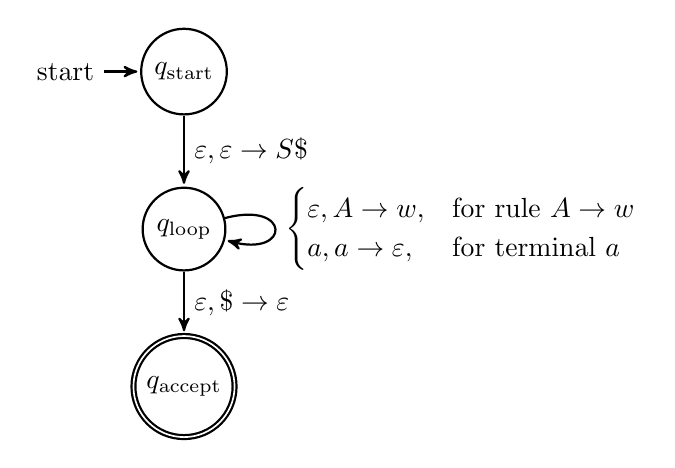
\begin{tikzpicture}[->,>=stealth',shorten >=1pt,auto,node distance=2cm,
			thick,base node/.style={circle,draw,minimum size=16pt}, real node/.style={double,circle,draw,minimum size=35pt}]

			\node[initial, state] (1) {$q_{\text{start}}$};
			\node[state] (2) [below of=1] {$q_{\text{loop}}$};
			\node[state, accepting] [below of=2] (3) {$q_{\text{accept}}$};

			\path[]
			(1) edge node {$\varepsilon, \varepsilon \to S\$$ } (2)
			(2) edge node {$\varepsilon, \$ \to \varepsilon$ } (3)
			(2) edge [loop right] node {$\begin{cases}\varepsilon, A \to w, & \text{for rule } A \to w\\ a, a \to \varepsilon, & \text{for terminal }a\end{cases}$} (2);
			
		\end{tikzpicture}
	\end{center}

	“$\Leftarrow$”: 需要根据 PDA 来构造 CFG. 不妨假设\footnote{需要简短地说明转化的可行性. 前两条只需要添加额外的结束状态和转移函数即可, 第三条需要在所有 both 和 neither 的转移中间插入中间状态.}该 PDA 有如下特性:\num{i}只有一个接受态$q_{\text{accept}}$, \num{ii}会在接受前清空栈, \num{iii}每次转移都会要么 push 要么 pop, 没有 both 和 neither 的情况. 构造变量$A_{pq}$表示所有能够使 PDA 从“状态$p$且栈空”转移到“状态$q$且栈空”的串组成的语言, 其中$A_{q_0q_{\text{accept}}}$是该 CFG 的起始变量. 按如下方式构造 CFG 的规则集合:
	\begin{itemize}
		\item 对于任意$p, q, r, s \in Q, u \in \Gamma, a, b \in \Sigma_{\varepsilon}$, 如果$(r, u) \in \delta(p, a, \varepsilon), (q, \varepsilon) \in \delta(s, b, u)$, 就添加规则$A_{pq} \to a A_{rs} b$, 
		\item 对于任意$p, q, r \in Q$, 添加规则$A_{pq} \to A_{pr}A_{rq}$, 
		\item 对于任意$p \in Q$, 添加规则$A_{pp} \to \varepsilon$. 
	\end{itemize}

	构造思路来源于考虑压栈弹栈的括号序列, 该序列要么被一个大括号包裹(第一种), 要么由两个括号序列组成(第二种). 可以归纳证明 $A_{pq}$ 的构造方式与其含义的等价性. 
\end{proof}
\begin{theorem}[Pumping Lemma for CFL]
	如果$A$是上下文无关语言, 那么存在一个数$p$(称为\obj{pumping length}), 使得对于任意$A$中长度至少为$p$的字符串$s$, $s$都可以分成五部分$s = uvxyz$满足
	\begin{itemize}
		\item for each $i \ge 0, uv^ixy^iz \in A$,
		\item $|vy| > 0$,
		\item $|vxy| \le p$.
	\end{itemize}
\end{theorem}
\begin{proof}
	设$b$为规则中的最大“度数”, 即替换字符串的最大长度. 如果 parse tree 的树高是$h$(根的深度是 $0$), 那么生成的字符串长度至多为$b^h$. 

	取 pumping length $p$ 为$b^{|V|+1}$. 长度至少为$p$的串对应的 parse tree 树高至少为$|V| + 1$, 故存在一条“直链”上有至少$|V| + 1$个变量, 根据\obj{鸽巢原理}, 存在一个变量出现至少两次, 记为$R$, 那么对于$R$就可以无限复制或者把两次出现压缩成一次(如图). 

	为了满足第二个条件, 我们要求 parse tree 必须是"最简"的, 因为只有冗余的替换方式才会导致两次 $R$ 的出现之间没有任何字符实际生成.

	为了满足第三个条件, 取$R$为满足条件的“深度最大”的, 即两个$R$都出现在最底下$|V| + 1$层. 此时$|vxy|$对应上面的$R$的子树大小, 受深度限制不超过$b^{|V| + 1} = p$. 
	\begin{center}
		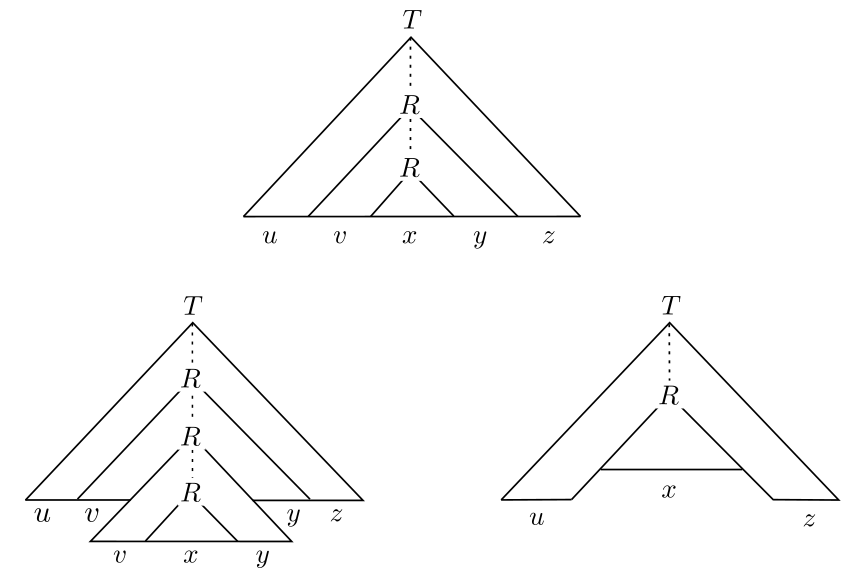
\includegraphics[scale=0.3]{pic/pumping_for_CFL.png}		
	\end{center}
\end{proof}
\begin{example}
	$B = \{a^nb^nc^n | n \ge 0\}$不是上下文无关语言.
\end{example}
\begin{proof}
	假设 B 是正则语言, 那么就存在 pumping length $p$. 考虑串 $a^pb^pc^p$, 注意到 $|vxy| \le p$ 故不可能含有超过两种字符, 那么在重复时就不可能保证三种字符出现次数仍然相同, 从而 $B$ 不是上下文无关语言.
\end{proof}
\begin{example}
	$C = \{a^ib^jc^k | 0 \le i \le j \le k\}$ 不是上下文无关语言.
\end{example}
\begin{proof}
	考虑串 $a^{p}b^{p}b^{p}$, 注意 $v, y$ 分别只能包含一种字符, 否则就会出现顺序错乱. 无论分别包含什么字符, 考虑 pumping up 或者 pumping down, 总可以使得生成的新字符串不属于 $C$, 从而 $C$ 不是上下文无关语言.
\end{proof}
\begin{example}
	$D = \{ww | w \in \{0, 1\}^*\}$ 不是上下文无关语言. 
\end{example}
\begin{proof}
	考虑 $s = 0^p1^p0^p1^p$. 

	首先指出 $vxy$ 必须跨域 $s$ 的中点. 假设 $vxy$ 只出现在 $s$ 的左半边, 那么 $uv^2xy^2z$ 中, 中点右侧的字符一定是 $1$(因为 $|vy| \le p$, 只会把 $\frac{|vy|}{2} \le \frac p2$ 个 $1$ 推到右半边), 而起始字符是 $0$ 说明该串不是 $ww$ 形式的. 

	但如果 $vxy$ 跨越 $s$ 的中点, 那么就一定跟前 $p$ 个 $0$ 与后 $p$ 个 $1$ 无交, 因此 $uxz$ 就会形如 $0^p1^i0^j1^p$, 其中 $i, j < p$, 这显然不属于 $D$.
\end{proof}

\newpage
\section{图灵机}

\begin{definition}[(Deterministic Turing Machine, TM)]
	(确定性)图灵机是一个七元组 $(Q, \Sigma, \Gamma, \delta, q_0, q_{\text{accept}}, q_{\text{reject}})$, 其中
	\begin{itemize}
		\item $Q$ 是状态集.
		\item $\Sigma$ 是不包含空格符$\Box$的输入字符集, $\Gamma$ 是纸带字符集. $\Sigma \subseteq \Gamma$.
		\item $\delta: Q \times \Gamma^k \to Q \times \Gamma^k \times \{L, S, R\}^k$ 是转移函数.
		\item $q_0, q_{\text{accept}}, q_{\text{reject}}$ 分别是起始态, 接受态和拒接态.
	\end{itemize}

	输入字符串写在第一条纸带的开头, 之前有一个 $\triangleright$ 作为起始表示.

	当图灵机运行到 $q_{\text{accept}}$ 或者 $q_{\text{reject}}$ 时, 会停机. 因此可以将其看成一个 $\Sigma^* \to \{0, 1\}$ 的函数. 一般地, 对于图灵机 $M$ 和字符串 $x \in \Sigma^*$, 我们有 $M(x) \in \{0, 1\}$, 称 $M(x) = 1$ 如果对于输入 $x$ $M$ 会到达接受态, 称 $M(x) = 0$ 如果对于输入 $x$ $M$ 会到达拒绝态\obj{或者不停机}.

	一个 \obj{configuration} 包含当前所在状态, 当前所有纸带上的信息, 和当前所有纸带头的位置. 称图灵机 $M$ 接受字符串 $w$, 如果存在一个 configuration 序列 $C_0, C_1, \cdots, C_t$ 满足 \num{i} $C_0$ 是起始 configuration, \num{ii} 每个 $C_i$ 都在一步内跳转到 $C_{i+1}$, \num{iii} $C_t$ 是接受 configuration.
\end{definition}
\begin{definition}[图灵可识别与图灵可判定]
	称一个语言是\obj{图灵可识别(Turing-recognizable)}的, 如果存在一台图灵机可以识别它(i.e. 接受其中的每一个字符串). 称一台图灵机是一个 \obj{decider}, 如果它对于任何输入都不会无限循环. 称一个语言是\obj{图灵可判定(Turing-decidable)}的, 如果存在一台 decider 可以识别它.
\end{definition}
\begin{definition}[函数的计算, 运行时间]
	考虑函数 $f: \{0,  1\}^* \to \{0, 1\}^*$ 以及 $T: \mathbb{N} \to \mathbb{N}$, 令 $M$ 为一图灵机. 我们称 $M$ 计算了函数 $f$, 如果对于任意 $x \in \{0, 1\}^*$, 只要 $M$ 的输入被初始化为$x$, 它就能在输出“输出纸带”上写下 $f(x)$ 并停机. 称 $M$ 在 $T(n)$ 的时间内计算了 $f$, 如果它计算每个 $x$ 都可以在 $T(|x|)$ 步内停机.
\end{definition}
\begin{definition}[Time-constructible functions]
	称一个函数 $T: \mathbb N \to \mathbb N$ 是 time-constructible的, 如果 $T(n) \ge n$ 且存在运行时间为 $T(n)$ 的计算函数 $x \to \rep{T(|x|)}$ 的图灵机 $M$, 其中 $\rep{x}$ 表示 $x$ 的 binary representation.
\end{definition}
\begin{example}
	$A = \{w \# w | w \in \{0, 1\}^*\}$ 可以被(单纸带)图灵机识别.
\end{example}
\begin{proof}
	给待匹配的两个位置打上标记, 每次前后移动找标记, 用状态记录已经看过的字符, 若比较失败则直接 reject, 否则向后移动标记继续比较直到全部比完. 以上的描述的图灵机的运行时间是 $T(n) = O(n^2)$ 的.
\end{proof}
\begin{example}
	$B = \{ww | w \in \{0, 1\}^*\}$ 可以被双纸带图灵机识别.
\end{example}
\begin{proof}
	\textit{没有 \# 记号, 无法方便地找到中间位置.} 可以在二号纸带上把输入复制一遍, 然后二号纸带头移动到中间(一号纸带头走一步, 二号纸带头走两步), 顺序比较即可. 运行时间是 $O(n)$.
\end{proof}

图灵机由字符集大小, 纸带数量等的不同, 产生了许多不同的变种. 它们在计算能力上会有所不同吗?

\begin{proposition}[大字符集规约到小字符集]
	对于任意$f: \{0, 1\}^* \to \{0, 1\}$以及time-constructible function $T: \mathbb{N} \to \mathbb{N}$, 如果$f$可以被图灵机$M$以$T(n)$时间计算, 那么它也可以被一台字符集为$\{0, 1, \Box, \triangleright\}$的图灵机$\tilde{M}$以$O(T(n)\log |\Gamma|)$的时间计算. 
\end{proposition}
\begin{proof}
	任意 $\Gamma$ 中的字符都可以用 $\log |\Gamma|$ 个比特表示. 每步转移时先用 $\log |\Gamma|$ 步读出纸带上一个字符的 encoding 并存入状态, 再根据转移函数进行移动, 最后用 $\log |\Gamma|$ 步写下新字符的 encoding 表示.
\end{proof}
\begin{proposition}[多纸带规约到单纸袋]
	对于任意$f: \{0, 1\}^* \to \{0, 1\}$以及time-constructible function $T: \mathbb{N} \to \mathbb{N}$, 如果$f$可以被有$k$条纸带的图灵机$M$以$T(n)$时间计算, 那么它也可以被一台单纸带图灵机$\tilde{M}$以$O(kT^2(n))$的时间计算. 单纸带指的是只有一条可读可写的纸带, 它同时扮演了输入、工作和输出纸带的角色. 
\end{proposition}
\begin{proof}
	把单条纸带上的位置按照模 $k$ 余数分配给 $k$ 条纸带, 对每种字符 $a$ 新建字符 $\hat a$ 表示所在纸带的纸带头指向这个字符. 注意到运行时间 $T(n)$ 的图灵机, 对于长度为 $n$ 的输入, 最多只会用到前 $T(n)$ 个位置, 所以每步转移时花费 $O(T(n))$ 的代价搜索每个纸带头的位置, 运行时间为 $O(kT^2(n))$.
\end{proof}
\begin{remark}[健忘的图灵机, oblivious Turing Machine]
	头部移动与输入长度有关, 而与输入的具体内容无关, 即对于任意$x \in \{0, 1\}^*$以及$i \in \mathbb N$, $M(x)$执行到第$i$步时读写头的位置是只关于$|x|$和$i$的函数. 可以证明图灵机可以平方规约到健忘的图灵机. 
	\label{oblivious}
\end{remark}
\begin{proposition}[双向图灵机规约到单向图灵机]
	对于任意$f: \{0, 1\}^* \to \{0, 1\}$以及time-constructible function $T: \mathbb{N} \to \mathbb{N}$, 如果$f$可以被双向图灵机(纸带的两个方向都有无限长)$M$以$T(n)$时间计算, 那么它也可以被一台单向图灵机$\tilde{M}$以$O(T(n))$的时间计算. 
\end{proposition}
\begin{thesis}[Church-Turing Thesis]
	任何物理上可实现的计算设备都可以被图灵机实现. 
\end{thesis}
\begin{theorem}[通用图灵机存在]
	存在图灵机$\mathcal U$使得对于任意$x, \alpha \in \{0, 1\}^*$, $\mathcal U(x, \alpha) = M_{\alpha}(x)$, 其中$M_{\alpha}$为被$\alpha$表示的图灵机. 进一步地, 如果$M_{\alpha}$对于$x$在$T$步内停机, 则$\mathcal U(x, \alpha)$可以在$CT\log T$步内停机, 其中$C$是一个仅依赖于$M_{\alpha}$的字符集大小、纸袋条数、状态数的常数. 
\end{theorem}
\begin{proof}
	构造 $\mathcal U$ 为一台五纸带图灵机, 五条纸带分别为
	\begin{itemize}
		\item Input, 被模拟图灵机 $M$ 的输入.
		\item Description of $M$, 主要是转移函数 $\delta$.
		\item Simulation of $M$, 记录纸带信息. 这里需要把 $M$ 规约成单纸带, 因而会产生平方的 overhead.
		\item Current state of $M$, 这部分不能简单地存在 $\mathcal U$ 的状态里, 因为对于 $\mathcal U$ 来说这不是常数.
		\item Output, $M$ 的输出.
	\end{itemize}

	注意每步模拟的过程中, 读取 $M$ 所在状态, 读取转移函数都是关于 $n$ 常数时间的.

	可以设计一种类似势能分析的算法, 把多纸带规约单纸带的 overhead 降到 $O(n \log n)$, 从而使通用图灵机模拟的复杂度优化到 $O(T \log T)$.
\end{proof}

\newpage
\section{不可判定语言}
\begin{definition}[可识别语言(Recognizable Language), 可判定语言(Decidable Language)]
	可识别语言就是能够被一台图灵机识别的语言. 可判定语言就是能够被一台 decider 识别的语言.
\end{definition}
\begin{theorem}
	存在不可识别语言.
\end{theorem}
\begin{proof}
	只需要考虑“语言”与“可识别语言”的基数. 前者的基数是 $2^{\aleph_0} = \aleph_1$, 后者的基数不超过图灵机的基数(因为存在可识别语言到图灵机的单射), 而图灵机可以被有限长的字符串描述, 因此是可数的.
\end{proof}
\begin{definition}[可计算函数(Computable Function)]
	可计算函数就是可以被一台图灵机计算的函数. 特别的, 考虑函数 $f: \{0, 1\}^* \to \{0, 1\}$, 则 $f$ 是可计算函数当且仅当 $L = \{x \in \{0, 1\}^*| f(x) = 1\}$ 是可判定语言.
\end{definition}
\begin{theorem}
	存在不可计算函数/存在不可判定语言.
\end{theorem}
\begin{proof}
	假设存在一个映射$\alpha \to M_{\alpha}$可以把任意字符串映到一台图灵机(以任意格式编码, 再把非法格式的串映到某台特定的图灵机即可). 考虑函数 $\text{UC}(\alpha) = 1 - M_{\alpha}(\alpha)$, 我们指出 $\text{UC}$ 是不可计算函数.

	假设 $\text{UC}$ 可计算, 考虑计算 $\text{UC}$ 的图灵机 $M$. 考虑 $\text{UC}(\rep{M})$, 由于 $M$ 计算了 $\text{UC}$, 我们知道 $\text{UC}(\rep{M}) = M(\rep M)$, 但根据 $\text{UC}$ 的定义, 又有 $\text{UC}(\rep M) = 1 - M(\rep M)$, 产生了矛盾.
\end{proof}
\begin{example}[停机问题不可判定]
	$\textsf{HALT} = \{\langle \rep M, \alpha \rangle | M \text{ halts on } \alpha\}$ 是不可判定语言.
\end{example}
\begin{proof}
	假设存在 $M_{\textsf{HALT}}$ 可以判定 $\textsf{HALT}$.
	
	利用 $M_{\textsf{HALT}}$ 可以构造判定语言 $L = \{\alpha | \text{UC}(\alpha) = 1\}$ 的 decider: 计算 $M_{\textsf{HALT}}(\langle \alpha, \alpha \rangle)$, 如果得到 $0$ (说明 $M_{\alpha}$ 对 $\alpha$ 不停机) 则直接输出 $1$, 否则输出$M_{\alpha}(\alpha)$ 的结果. 这与 $\text{UC}$ 不可计算相矛盾. 因此 \textsf{HALT} 不可判定.
\end{proof}
\begin{example}[接受问题不可判定]
	$\textsf{AC} = \{\langle \rep M, \alpha \rangle | M \text{ accepts } \alpha\}$ 是不可判定语言.	
\end{example}
\begin{proof}
	利用 $M_{\textsf{AC}}$ 可以直接构造 $M_{\text{UC}}$: 只要把 $M_{\textsf{AC}}(\langle \alpha, \alpha \rangle)$ 的输出取反即可.
\end{proof}
\begin{definition}[映射规约, Mapping Reduction]
	称语言 $A$ 可映射规约到(is mapping reducible to) 语言 $B$, 如果存在可计算函数 $f: \Sigma^* \to \Sigma^*$, 使得 $w \in A$ 当且仅当 $f(w) \in B$, 记作 $A \le_m B$.
\end{definition}
\begin{proposition} 如果 $A \le_m B$, 则
	\begin{itemize}
		\item 如果 $B$ 可判定, 则 $A$ 也可判定.
		\item 如果 $A$ 不可判定, 则 $B$ 也不可判定.
	\end{itemize}
\end{proposition}
\begin{example}
	$\textsf{NAC} = \{\rep M | M \text{ accept nothing}\}$ 是不可判定语言.
\end{example}
\begin{proof}
	考虑构造映射 $f$ 满足 $w \in \overline{\textsf{AC}} \Leftrightarrow f(w) \in \textsf{NAC}$. 令 $f(\langle \rep M, \alpha \rangle) = \rep{M'}$ 其中 $M'$ 不管输入直接运行 $M(\alpha)$. $f$ 显然是可计算的, 故 $\overline{\textsf{AC}} \le_m \textsf{NAC}$, 而可判定语言关于补集的封闭性导致 $\overline{\textsf{AC}}$ 是不可判定语言, 从而 $\textsf{NAC}$ 是不可判定语言.
\end{proof}
\begin{example}
	$\textsf{EQU} = \{\langle \rep{M_1}, \rep{M_2} \rangle | L(M_1) = L(M_2)\}$ 是不可判定语言.
\end{example}
\begin{proof}
	考虑构造映射 $g$. 取 $g(\rep{M}) = \langle \rep{M}, \rep{M'}\rangle$ 其中 $M'$ 是拒绝一切输入的图灵机. 于是 $\rep{M} \in \textsf{NAC} \Leftrightarrow \langle \rep{M}, \rep{M'}\rangle \in \textsf{EQU}$, $\textsf{NAC} \le_m \textsf{EQU}$, 从而 \textsf{EQU} 是不可判定语言.
\end{proof}
\begin{theorem}
	语言 $A$ 可判定当且仅当 $A$ 与 $\overline{A}$ 均可识别.
\end{theorem}
\begin{proof}
	$\Rightarrow$: 显然.

	$\Leftarrow$: 记 $A$ 可被 $M_1$ 识别, $\overline A$ 可被 $M_2$ 识别, 考虑\obj{并行}运行 $M_1$ 和 $M_2$, 总有一个会给出结果. 
\end{proof}
\begin{corollary}
	\textsf{HALT} 和 \textsf{AC} 都是不可判定的可识别语言. 这说明 $\overline{\textsf{HALT}}$ 和 $\overline{\textsf{AC}}$ 都是不可识别语言.
\end{corollary}

\newpage
\section{时间复杂性, \P 与 \NP}
\begin{definition}[\DTIME 与 \P]
	对于函数$T: \mathbb N \to \mathbb N$, 称语言$L \in \DTIME(T(n))$, 如果存在常数$c > 0$和一台运行时间为$c \cdot T(n)$的图灵机可以决定$L$. 

	$\P = \bigcup_{c \ge 1}\DTIME(n^c)$. 
\end{definition}
\begin{proposition}
	$\P$ 在多项式次集合操作下是封闭的.
\end{proposition}
\begin{example}
	$\textsf{PATH} = \{ \langle G, s, t\rangle : G \textrm{ is a direct graph in which there is a path from }s \textrm{ to } t\} \in \P.$
\end{example}
\begin{theorem}[Time Hierarchy Theorem]
	$f, g$是满足$f(n) \log f(n) = o(g(n))$的time constructible的函数, 则
	$$\DTIME(f(n)) \subsetneq \DTIME(g(n))$$
	\label{time_hierarchy_thm}
\end{theorem}
\begin{proof}
	考虑这样的图灵机$D$:对于$x \in \{0, 1\}^*$, 用通用图灵机$\mathcal{U}$模拟$M_x(x)$运行至多$g(|x|)$步(是$\mathcal U$的$g(|x|)$步而不是$M_x$的$g(|x|)$步), 如果$\mathcal{U}$在$g(|x|)$步数内输出了$b \in \{0, 1\}$, 则$D$输出$1-b$, 否则$D$输出$0$. 

	根据定义, $D$对于任何输入$x$都会在$g(|x|)$步内停机, 因此$L(D) \in \DTIME(g(n))$. 我们通过反证法证明$L(D) \notin \DTIME(f(n))$. 先叙述否命题: 存在图灵机$M$和常数$c$, 使得对于任意输入$x \in \{0, 1\}^*$, $M$都能在$cf(|x|)$步内输出与$D$相同的结果. 

	对于输入$x$, 用通用图灵机$\mathcal{U}$模拟$M$只需要$c'cf(|x|)\log f(|x|)$步, 其中$c'$是不依赖于$|x|$的一个常数. 由于$f(n) \log f(n) = o(g(n))$\footnote{little-$o$不能替换成big-$O$, 我只能说懂的都懂. }, 故存在充分大的$n_0$使得$g(n) > c'cf(n) \log f(n)$对于任意$n \ge n_0$均成立. 令$x' = \rep{M}$ 满足 $|x'| \ge n_0$, 那么
	\begin{itemize}
		\item $D$会输出与$M$相同的结果, 因为这是$M$的定义;
		\item $D$会输出与$M$不同的结果, 因为$c'cf(n)\log f(n) < g(n)$使得$\mathcal U$对$M$的模拟已经结束了, 根据$D$的定义, $D$应该输出相反的结果. 
	\end{itemize}

	产生了矛盾. 因此$\DTIME(f(n)) \subsetneq \DTIME(g(n))$. 
\end{proof}
\begin{definition}[\NP]
	称语言$L \subseteq \{0, 1\}^*$属于\NP, 如果存在一个多项式$p: \mathbb N \to \mathbb N$和一个多项式时间图灵机$M$(称其为$L$的\obj{verifier})使得对于任意的$x \in \{0, 1\}^*$, 都有
	$$x \in L \Leftrightarrow \exists u \in \{0, 1\}^{p(|x|)}, M(x, u) = 1$$
	如果$x \in L$与$u \in \{0, 1\}^{p(|x|)}$满足$M(x, u) = 1$, 则称$u$是$x$的一个\obj{certificate}. 
\end{definition}
\begin{proposition}
	定义$\EXP = \bigcup_{c > 1} \DTIME(2^{n^c})$, 则$\P \subseteq \NP \subseteq \EXP$. 
\end{proposition}
\begin{remark}
	根据 Time Hierarchy Theorem 我们知道 $\P \subsetneq \EXP$, 因此 $\P \subsetneq \NP$ 与 $\NP \subsetneq \EXP$ 至少一者为真.
\end{remark}
\begin{definition}[非确定图灵机与\NTIME]
	非确定图灵机(Nondeterministic Turing Machine, NDTM)是有两个转移函数$\delta_0, \delta_1$和一个特定状态$q_{\text{accept}}$的图灵机$M$, 每步转移时, 可以任意选择遵从某一个转移函数. 对于输入$x$, 称$M(x) = 1$当且仅当存在一个选择序列可以使$M$到达$q_{\text{accept}}$状态, 否则——任意选择序列都无法在停机前到达$q_{\text{accept}}$——就认为$M(x) = 0$. 称$M$的运行时间为$T(n)$, 如果对于任意输入$x \in \{0, 1\}^*$以及任意的选择序列, $M$都会在$T(|x|)$步内到达$q_{\text{accept}}$或者$q_{\text{halt}}$. 

	对于$T: \mathbb N \to \mathbb N$和语言$L \subseteq \{0, 1\}^*$, 称$L \in \NTIME(T(n))$, 如果存在常数$c > 0$和一个运行时间为$c \cdot T(n)$的非确定图灵机$M$, 满足对于任意的$x \in \{0, 1\}^*$, $x \in L \Leftrightarrow M(x) = 1$. 
\end{definition}
\begin{theorem}
	$\NP = \bigcup_{c \ge 1} \NTIME(n^c)$. 
\end{theorem}
\begin{proof}
	非确定图灵机的选择序列可以看作$x$的一个 certificate, 反之亦然. 
\end{proof}


\begin{definition}[多项式时间规约, \NP-hard 与 \NP-complete]
	称语言$L \subseteq \{0, 1\}^*$可\obj{多项式时间(Karp)规约}到语言$L' \subseteq \{0, 1\}^*$(记作$L \le_p L'$), 如果存在一个多项式时间可计算函数$f: \{0, 1\}^* \to \{0, 1\}^*$使得对于任意$x \in \{0, 1\}^*$, $x \in L \Leftrightarrow f(x) \in L'$. 

	称$L' \in $ \NP-hard, 如果对于任意$L \in \NP$, $L \le_p L'$. \NP-complete $=$ \NP\ $\cap$ \NP-hard.  
\end{definition}
\begin{theorem}[$\le_p$的传递性]
	\begin{itemize}
		\item 若$L \le_p L'$且$L' \le_p L''$, 则$L \le_p L''$. 
		\item 如果$L \in $ \NP-hard, 则$L \in \P \Rightarrow \P = \NP$. 
		\item 如果$L \in $ \NP-complete, 则$L \in \P \Leftrightarrow \P = \NP$. 
	\end{itemize}
\end{theorem}
\begin{theorem}[Cook-Levin Theorem]
	$\textsf{SAT}, \textsf{3SAT} \in $ \NP-complete. 

	其中 $\textsf{SAT} = \{\varphi \in \text{CNF} | \varphi \text{ is satisfiable}\}, \textsf{3SAT} = \{\varphi \in 3\text{CNF} | \varphi \text{ is satisfiable}\}$. CNF(Conjunctive Normal Form, 合取范式)是一种形如 $\bigwedge_i\left(\bigvee_j v_{i_j}\right)$ 的特殊的 boolean formula.
\end{theorem}
\begin{proof}
	$\textsf{SAT}, \textsf{3SAT} \in \NP$ 是平凡的. 先考虑证明 $\textsf{SAT} \in \NP$-hard, 即 $\forall L \in \NP, L \le_p \textsf{SAT}$. 回顾两者定义
	\begin{center}		
		\begin{tabular}{cccc}
			$\varphi_x \in \textsf{SAT}$ & $\Leftrightarrow$ & $\exists$ assignment $u$ & s.t. $\varphi_x(u) = \text{True}$\\
			$x \in L$ & $\Leftrightarrow$ & $\exists$ certificate $u$ & s.t. $M(x, u) = 1$\\
		\end{tabular}
	\end{center}
	因此考虑根据 $M, x$ 来构造\obj{多项式规模的} $\varphi_x$, 满足 $M(x, u) = 1 \Leftrightarrow \varphi_x(u) = \text{True}$. 
	
	不妨假设 $M$ 是 \num{i} 双纸带且第一条纸带只读 \num{ii} oblivious 的(参见\cref{oblivious}), 那么在$M$运行到第 $i$ 步时, 其两个纸带头所指向的符号, 当前状态所组成的三元组 $z_i \in \Gamma \times \Gamma \times Q$ (称之为 $M$ 运行到第 $i$ 步时的 \obj{snapshot})将由后三者唯一决定: $z_{i-1}, z_{\text{prev}(i)}$ 和 $(x \circ u)_{\text{inputpos}(i)}$, 其中 $\text{prev}(i)$ 表示上一次与第$i$步访问到工作纸带相同位置的时刻, $\text{inputpos}(i)$ 表示第 $i$ 步时访问到输入纸带的位置.

	根据 $M$ 的转移函数 $\delta$, 可以构造出 $F: \{0, 1\}^{2c+1} \to \{0, 1\}^c$ 满足 $z_i = F(z_{i-1}, z_{\text{prev}(i)}, (x \circ u)_{\text{inputpos}(i)})$, 其中 $c$ 是表示一个 snapshot 所需的比特数. 

	可以构造一个有 $n + p(n) + cT(n)$ 个变量的 CNF $\varphi_x$, 这些变量分别记为 $y$ 以及 $z_1, \cdots, z_{T(n)}$, 它是下述这些条件的 AND:
	\begin{enumerate}
		\item $y$ 的前 $n$ 位和 $x$ 相同.
		\item $z_1$ 表示初始状态 $(\triangleright, \Box, q_{\text{start}})$.
		\item $z_i = F(z_{i-1}, z_{\text{prev}(i)}, y_{\text{inputpos}(i)}) \ (\forall i \in \{2, \cdots, T(n)\})$.
		\item $z_{T(n)}$ 表示到达 $q_{\text{halt}}$ 的终止状态.
	\end{enumerate}

	这些条件用 CNF 表示出来, 其长度是 $d(n + T(n))$, 其中 $d$ 是与 $n$ 无关的常数. 从而我们实现了多项式时间规约, 完成了 $L \le_p \textsf{SAT}$ 的证明.

	然后考虑证明 $\textsf{SAT} \le_p \textsf{3SAT}$. 只需要注意到
	$$\bigvee_{i=1}^{k}u_i \cong \left(z \vee \bigvee_{i=1}^{k-2}u_i\right) \wedge (\overline{z} \vee u_{k-1} \vee u_{k})$$
	说明任意 CNF 都可以多项式时间规约到 3CNF. 所以 $\textsf{SAT} \le_p \textsf{3SAT}$.
\end{proof}


\newpage\vspace*{\fill}\begin{center}\textit{后面都是自己瞎写的阿拉丁.}\end{center}\vspace*{\fill}

\begin{theorem}[Nondeterministic Time Hierarchy Theorem]
	$f, g$是满足$f(n + 1) = o(g(n))$的time constructible的函数, 则
	$$\NTIME(f(n)) \subsetneq \NTIME(g(n))$$
\end{theorem}
\begin{theorem}[Ladner's Theorem]
	如果$\P \neq \NP$, 则存在语言$L \in \NP \setminus \P$, 即非 \NP-complete 的 \NP 语言. 
\end{theorem}

\newpage
\section{空间复杂性}
\begin{definition}[运行空间, \SPACE 与 \NSPACE]
	对于$S: \mathbb N \to \mathbb N$和$L \subseteq \{0, 1\}^*$, 称$L \in \SPACE(S(n))$, 如果存在常数$c$以及可以决定$L$的图灵机$M$, 满足在对任意长度为$n$的输入的计算中, $M$只会访问到至多$c \cdot S(n)$个work tapes上(不包含input)的位置, 称$M$的运行空间为$O(S(n))$. 

	类似地可以定义$\NSPACE$, 这里要求在任何一种决策下用到的位置数量都不超过$c \cdot S(n)$. 
\end{definition}
\begin{definition}[Space constructible functions]
	称$S: \mathbb N \to \mathbb N$是space constructible的, 如果存在图灵机可以对于输入$x$, 在$O(S(|x|))$的空间内计算$S(|x|)$. 
\end{definition}
\begin{remark}
	相比于 time constructible functions, 我们不要求 space constructible functions 满足 $S(n) \ge n$, 但为了能够“记住在输入纸带上的位置”, 我们一般会要求 $S(n) \ge \log n$. 
\end{remark}
\begin{theorem}
	对于任何 space constructible 的函数$S: \mathbb N \to \mathbb N$, 有
	$$\DTIME(S(n)) \subseteq \SPACE(S(n)) \subseteq \NSPACE(S(n)) \subseteq \DTIME(2^{O(S(n))})$$
	\label{time_and_space}
\end{theorem}
\begin{proof}
	前两个$\subseteq$都是平凡的, 只考虑证明最后一个. 

	我们称一台(确定或非确定)图灵机$M$的一个\obj{configuration}包含\num{i}work tape上的所有非空字符;\num{ii}所有纸带的head位置;\num{iii}$M$所处的状态, 则对于确定的输入$x \in \{0, 1\}^*$, 一个configuration的后继configuration是\num{a}对于图灵机来说, 唯一确定的;\num{b}对于非确定图灵机来说, 至多唯二确定的. 把configuration之间的转移看成一张有向图, 记作$G_{M, x}$. 不失一般性假设$M$只有一种configuration $C_{\text{accept}}$满足“输出$1$后停机”(可以让图灵机在停机前擦除所有中间记录), 这样$M(x) = 1$就等价于$G_{M, x}$中存在一条$C_{\text{start}}$到$C_{\text{accept}}$的路径. 

	陈述两个事实:
	\begin{itemize}
		\item 给定$M, x$, $G_{M, x}$中的每个节点用$O(S(n))$个bit来表示, 也即, $G_{M, x}$只有$2^{O(S(n))}$个节点. 
		\item 对于任意两个configuration $C, C'$, 存在$O(S(n))$大小的CNF $\varphi_{M, x}$满足$\varphi_{M, x}(C, C') = 1$当且仅当$G_{M, x}$中$C$有边连向$C'$. 
	\end{itemize}

	因此用$2^{O(S(n))}$的时间把整张$G_{M, x}$建出来, 再 BFS 一下即可验证$C_{\text{start}}$到$C_{\text{accept}}$是否连通. 
\end{proof}
\begin{definition}[\PSPACE, \NPSPACE, \L \ and \NL]
	\begin{align*}
		\PSPACE &= \bigcup_{c \ge 1}\SPACE(n^c)\\
		\NPSPACE &= \bigcup_{c \ge 1}\NSPACE(n^c)\\
		\L &= \SPACE(\log n)\\
		\NL &= \NSPACE(\log n)
	\end{align*}
\end{definition}
\begin{corollary}
	$\NP \subseteq \PSPACE$, 因为都可以暴力枚举答案, 用多项式空间存下来然后验证. 
\end{corollary}
\begin{corollary}
	在 \cref{time_and_space} 中分别代入$S(n) = \log n, S(n) = n^c$, 可以得到
	$$\L \subseteq \P\qquad \PSPACE \subseteq \EXP$$
\end{corollary}
\begin{example}
	$$\textsf{PATH} = \{ \langle G, s, t\rangle : G \textrm{ is a direct graph in which there is a path from }s \textrm{ to } t\}$$
	即判断图中两点之间是否存在一条路径. 显然$\textsf{PATH} \in \NL$, 但其是否属于$\L$仍是一个open problem. 
\end{example}
\begin{theorem}[Space Hierarchy Theorem]
	$f, g$是满足$f(n) = o(g(n))$的 space constructible 的函数, 则
	$$\SPACE(f(n)) \subsetneq \SPACE(g(n))$$
\end{theorem}
\begin{proof}
	技术细节在于通用图灵机$\mathcal U$模拟图灵机$M$只需要常数倍的空间, 所以相比于 Time Hierarchy Theorem 没有了对数项. 其余部分跟 Time Hierarchy Theorem 的证明类似, 就不再赘述了. 	
\end{proof}
\begin{definition}[\PSPACE-hard, \PSPACE-complete]
	称$L'$是\PSPACE-hard, 如果对于任意$L \in \PSPACE$, $L \le_p L'$. \PSPACE-complete $=$ \PSPACE\ $\cap$ \PSPACE-hard.  
\end{definition}
\begin{example}
	$$\textsf{SPACE TMSAT} = \{ \langle M, w, 1^n \rangle : \textrm{DTM } M \textrm{ accepts } w \textrm{ in space } n \}$$
	这是一个 \PSPACE-complete 语言. 
\end{example}
\begin{definition}[Quantified Boolean formula, QBF]
	一个 QBF 是形如 $Q_1x_1Q_2x_2 \cdots Q_nx_n \varphi(x_1, x_2, \cdots, x_n)$ 的公式, 其中$Q_i \in \{\forall, \exists\}$, $x_i$的取值是$\{0, 1\}$, $\varphi$是一个 plain(unquantified) boolean formula . 

	上述定义专注于讨论\obj{前束范式}的 QBF , 因为非前束范式都可以转化成等价的前束范式. 一个 QBF 有真值 true 或 false . 

	用 \textsf{TQBF} 表示所有为真的 QBF 的集合. 
\end{definition}
\begin{theorem}
	\textsf{TQBF} is \PSPACE-complete.
\end{theorem}
\begin{proof}
	先证明 $\textsf{TQBF} \in \PSPACE$. 这个是简单的, 因为判定可以通过 dfs 实现, 而 dfs 只需要$O(n + m)$的空间, 其中$n$是变量数, $m$是 QBF 的长度. 

	再证明任意$L \in \PSPACE$都满足$L \le_p \textsf{TQBF}$. 假设$M$是在$S(n)$空间内计算$L$的图灵机, 考虑输入$x \in \{0, 1\}^*$. 考虑 configuration graph $G_{M, x}$, 我们陈述过图中每个点可以用$m = O(S(n))$个bit来表示, 以及存在一个 CNF $\varphi_{M, x}$ 满足$\varphi_{M, x}(C, C') = \textrm{true}$ 当且仅当$G_{M, x}$ 中有 $C \to C'$ 的边. 

	考虑根据 $\varphi_{M, x}$ 来构造我们想要的 QBF $\psi$ . 用 $\psi_i$ 表示一个 QBF , $\psi_i(C, C') = \textrm{true}$当且仅当$G_{M, x}$中存在一条长度不超过$2^i$从$C$到$C'$的路径, 那么显然$\psi = \psi_m(C_{\text{start}}, C_{\text{accept}}), \psi_0(C, C') = \varphi_{M, x}(C, C') \vee (C = C')$. $\psi_i$可以递归定义:对于$i \ge 1$, $\psi_i(C, C') = \exists C'' \psi_{i-1}(C, C'') \wedge \psi_{i-1}(C'', C')$. 

	一个技术细节是需要改进递归定义的具体方式以保证$\psi$的长度是多项式级别的. 可以用一种看上去有点奇怪, 但与前述定义等价的形式:
	$$\psi_i(C, C') = \exists C''\forall D_1 \forall D_2 ((D_1, D_2) = (C, C'') \wedge (D_1, D_2) = (C'', C')) \Rightarrow \psi_{i-1}(D_1, D_2)$$

	这样构造出的 QBF $\psi$ 的长度是$O(m^2) = O(S^2(n))$的. 
\end{proof}

\end{document}
